\documentclass[a4paper]{article}
\usepackage{tgbonum}
%% Language and font encodings
\usepackage[english]{babel}
\usepackage[utf8x]{inputenc}
\usepackage[T1]{fontenc}
\usepackage{tikz}
\usepackage{soul}
\setlength{\parskip}{1em}

%% Sets page size and margins
\usepackage[a4paper,top=2.5cm,bottom=2.5cm,left=3cm,right=3cm,marginparwidth=1.75cm]{geometry}

%% Useful packages
\usepackage{amsmath}
\usepackage{amsthm}
\usepackage{amssymb}
\usepackage{hhline}
\usepackage{graphicx}
\usepackage{float}
\usepackage{tikz}
\usepackage{verbatim, enumerate}
\usepackage[colorinlistoftodos]{todonotes}
\usepackage[colorlinks=true, allcolors=blue]{hyperref}

\newcommand{\pois}[1]{\mathsf{Pois(}{#1}\mathsf{)}}

\title{\vspace{5cm}Starbucks Queue Modeling}
\author{Nuo Chen \\ Phoebe Hu \\
Tianhang Gao\\ Liangyu Zhao \\ [1.0 cm]
		University of Washington \\
		Math 381 Group 4 \\
        Instructor: Dr. Conroy}

\begin{document}

\begin{titlepage}
\maketitle
\end{titlepage}

{\hypersetup{linkcolor=black}
\tableofcontents
}

\newpage

\section{Introduction}
Waiting for things is a common scenario in other parts of the world, however, the American people are less tolerant about such thing. It's easy for us to get frustrated when the line is longer than your expectations or worse, sometimes when the line does not seem to move at all. However, the reduction of waiting time usually requires extra investment. For example, having more windows or training employees longer to have them work more efficiently. To see if the investment is actually worthy, and to accurately assess the wait time based on  we build up queuing models to evaluate the waiting time and number of customers. In this paper we simulated the waiting time and service routine at the recently renovated Suzzallo Starbucks Cafe using Monte Carlo method and queuing theory. The purpose of the study is to gain insights on questions such as 'How to reduce customer wait time with the least amount of change?', and 'How long do I have to wait to get my Triple, Venti, Soy, No Foam Latte.' To do so, we incorporated computer simulations to do the heavy lifting for us and established computational models for each part of the Starbucks' service routine using Python.  

\section{Background}

\subsection{Motivation}
Imagine the following scene, you are on your way to work the morning after a long, sleepless night of studying, all you want is cup of coffee to get yourself together. Then you notice there is a Starbucks around the corner. However, you soon realize that there are many others who are also in desperate need of some caffeine, and the line stretches all the way from the counter to the entrance. There is a conflict between your desire for a coffee and the waiting time you have to spend. Inspired by this daily conflict, we decide to model this process, so that people can have an estimate of their waiting time to help them rationalize their decisions. 

\subsection{Data Collection}
We make some questionnaires (see appendix for the survey result and data collected) to get data from reality. In our questionnaire we ask the staff of Suzzallo Starbucks the time it takes for them to make each beverage on our list and also the popularity of each beverage.\cite{ranking}  In particular, we firstly ask them the sale quantity of the least popular beverage and use its sale volume as one unit. Based on the unit, we then have the popularity from one to five. To be more specific, the sale quantity of the beverage of popularity level five is roughly five times more than the beverage of popularity level one. 

\subsection{Previous Research}
Similar problems in the past have been researched by other people. In particular, we find two similar researches in the past that primarily focused on Starbucks' Queuing model. 

There is an article "Starbucks waiting time and lean operation" by Shmula published in December 7, 2010 that models the Starbucks wait time. In the article, Shmula identified that arrival rate of customers at any restaurants/cafe usually follows a 'M/M/1' distribution, a special type of Poisson distribution with the following characteristics:\cite{analyzing}

\begin{itemize}
\item The costumer arrives randomly,
\item There is a random service,
\item only one service channel, in this case, one cashier. 
\end{itemize}

Shmula also assumes the average time to serve a customer is 3 minutes (include placing order, making drinks, and pickup drinks) and there are 2000 customers on a 12-hour day. He has variables of arrival rate, service rate, number of service channels and random arrival and deterministic service rate. Based on the model and the assumption, he gets the following result: The average time for a customer in a line is around 4 minutes and the average of the customer in the system is roughly 5 minutes. Average time to wait in the line is 12 minutes and the average waiting time in the system is 15 minutes. 
Our model shares some similarities with Shmula's. For example, both of us define the customer arrival rate to follow a "M/M/1" distribution. However, we take an empirical approach to obtain real world data through surveying Starbucks' employees. As mentioned previously, we make questionnaire to get the average making time for each of beverage and take that into consideration, instead of just assuming the time it takes to serve each customer is 3 minutes. When we generate the model to calculate the estimated waiting time, we consider that there is difference of making each beverage and we have the estimate probability of each beverage. 

There are some other slides online talking about Starbucks' queue.\cite{timing} There is an interesting one which analyzes the wait time people spent at the queue of Starbucks. Our model is different from theirs in the following aspect: 
\begin{itemize}
\item We used different queueing models for order placement and order processing.

\item We prioritizes items that takes the longest preparation time on top of the FIFO principle. 

\item They defined the waiting time to be influenced by 3 parameters, which are the day, the week and the time of arrival. 
\end{itemize}
In their conclusion, they find that the average time for a customer to wait is 4.21 minutes. Hence, in a year the customer will lose two full 8.5-hour work days by going to Starbucks. 

Based on the data we get from observation and guided by these two papers, we generate our model to best calculate the waiting time. 

\newpage
\section{Modeling}

For the purpose of the project, we decided to use Queuing Model and Monte Carlo simulation to study the wait time and processing capability at Starbucks. After gathering data through surveying store employees and observing customer behaviors at Suzzallo Starbucks, we have devised the following model that best captures customer interaction and order processing. For the simulation in Python, see the repository link in Appendix. (The actual code files are too large to be included as excerpts in the paper)

\begin{figure}[H]
	\centering
	\includegraphics[width=0.60\textheight]{GeneralModel}
	\caption{General Model}
\end{figure}

As shown in the figure 1, our model consists of four main parts. In the order of completing customer purchase, they are: customer queue model, order placement, order processing, and order pickup. Customer first arrives at the customer queue where he or she waits in queue to order the drinks with the cashier. The cashier will then place the order and submit it to the order processing part. The order processing part produces the drinks in the order. Once an order has been done, it is sent to the order pickup part for the customer to pickup.

The order placement and order processing are fixed while different customer queue models and pickup model will be applied for us to study their behaviors. Now, we go into each part of the model in details.

\subsection{Arrival Process}

In the arrival process, we need to simulate people arriving at Suzzallo Starbucks. There are three key components we need to decide in the random process: rate of customer arrival, number of items each customer will order, and the type of each item customer will order. We will discuss each one of them in the following sections. 

\subsubsection{Rate of Arrival}

As most of the queue models do, we use Poisson distribution $\pois{\lambda}$ to model our arrival process. The $\lambda$ here is the number of people arrive per second. To simulate the real arrival process, our $\lambda$ is designed not to be a constant, but vary dynamically based on the number of people currently in the queue. We assume $\lambda$ decrease exponentially as the number of people waiting increases. The precise formula is
\[\lambda=\lambda_0e^{-k\cdot N}\]
where $N$ is the number of people already in the model including people waiting for placing orders and picking up, $\lambda_0$ is the average rate of arrival when nobody is in the model, and $k$ is a positive constant we need to estimate.

\begin{figure}[H]
	\centering
	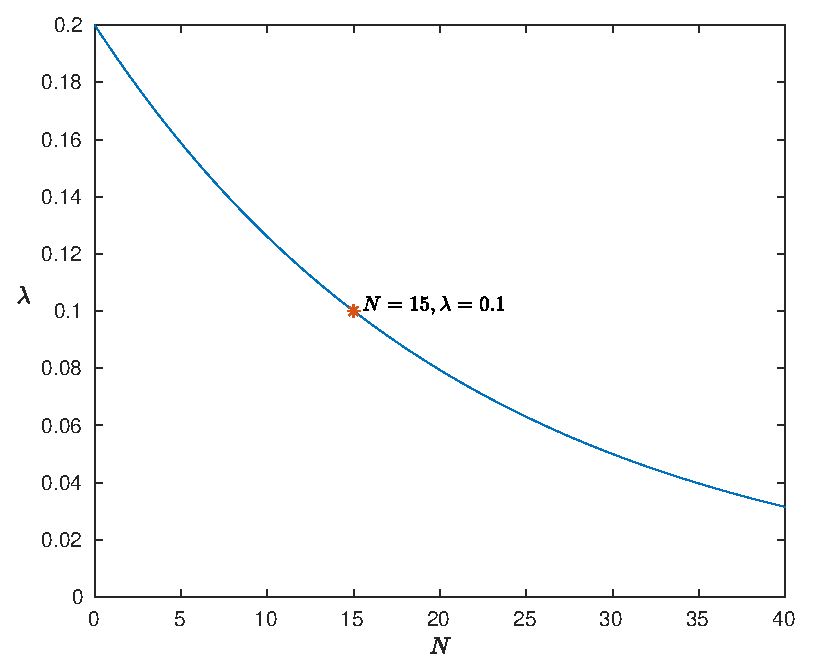
\includegraphics[width=0.35\textheight]{arrival_lambda}
	\caption{$\lambda$ vs $N$ when $\lambda_0=0.2,k=\frac{\log 2}{15}$}
\end{figure}

After spending an afternoon observing at the Suzzallo Starbucks, we found that during the class break, the peak rate of arrival is $\lambda_0=0.2$ (0.2 person per second) in average. Additionally, people tend to give up enqueuing when there are more than 30 people in the line. Assuming the rate of arrival will be halved at 15 people, we got a $k=\frac{\log 2}{15}$. Thus, we have a dynamic random process to simulate the arrival process with balking in which less people will enqueue when the queue is too long.

\subsubsection{Number of items}

For the number of items each customer will order, we also assume it satisfy Poisson distribution \mbox{$\pois{\lambda-1}+1$}, but this time we interpret $\lambda$ as the average number of items ordered per person. The reason why we take \mbox{$\pois{\lambda-1}+1$} instead of $\pois{\lambda}$ directly is because ordering zero items does not make any sense. Again, we observed 100 people at Suzzallo Starbucks, and here is the data we obtained:

\begin{center}
    \begin{tabular}{ c | c }
    	Number of Items Ordered & Count of Customers \\
    	\hline
        1 & 73 \\
        2 & 19 \\
        3 & 5 \\
        4 & 3
    \end{tabular}
\end{center}

Based on the data, we obtain an average number of items ordered per person $\lambda=1.38$.

\begin{figure}[H]
	\centering
	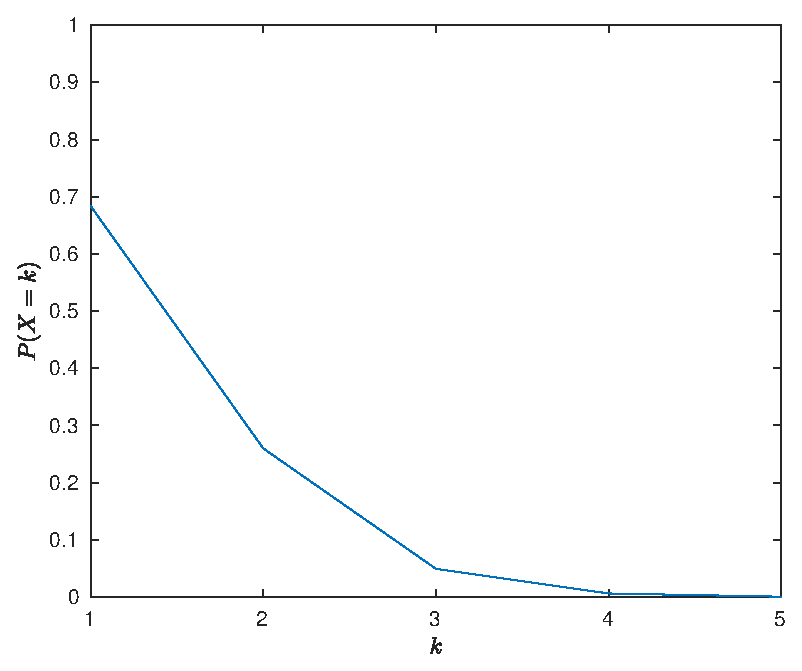
\includegraphics[width=0.35\textheight]{pois_dist}
	\caption{$\pois{1.38-1}+1$ probability mass function of ordering $k$ items}
\end{figure}

In fact, this probability mass function fits our data pretty well. The probability of ordering 1 item is near 70\% and 2 items is 20\%, which behaves similarly to our data.

\subsubsection{Type of item}

After deciding the number of items a customer will buy, we need to decide what each of the items is. To obtain a realistic simulation, the exact drink customer ordered will be chosen randomly based on each beverage's probability. For the list of drinks, we choose the top 17 popular drinks and surveyed Starbucks' employees for their preparation time and popularity. The reason why we only choose the top 17 is for simplicity. Most of the customers of Starbucks only order several types of drink, so the rest of the drinks are too trivial to have a significant influence on the model. Five employees at Suzzallo Starbucks have done the survey. Here is the averaged result:

\begin{center}
    \begin{tabular}{ l | c | c }
    	Drink & Preparation Time (s) & Popularity \\
        \hline
    	Latte&28&4\\
        Vanilla Latte&26&5\\
        Pumpkin Spice Latte&40&4.6\\
        Cappuccino&24&2.2\\
        Drip Coffee&10&3.2\\
        Mocha&36&4\\
        Pepermint Mocha&44&3.4\\
        White Chocolate Mocha&36&3.8\\
        Caramel Macchiato&44&4.4\\
        Hot Chocolate&26&3.8\\
        Chai Tea Latte&22&3.8\\
        Green Tea Latte&34&3.8\\
        Iced Coffee&10&3\\
        Iced Passion Tea&46&2.4\\
        Iced Green Tea Lemonade&66&3.2\\
        Italian Soda&78&1\\
        Pink Drink&58&5
    \end{tabular}
\end{center}

To assess the probability of a drink gets ordered, we decided to measure the popularity of the drink with numeric scale. Out of the 17 drinks, we find the least popular drink to be ``Italian Soda'' and use its popularity as a measurement unit (i.e Italian soda will have a popularity of 1, and if a drink is twice as popular as the Italian Soda, it will be assigned a popularity of 2). Therefore, the estimated probabilities are:

\begin{center}
    \begin{tabular}{ l | c }
    	Drink & Probability (rounded to 2 decimal points) \\
        \hline
		Latte & 6.60\% \\
		Vanilla Latte & 8.25\% \\
		Pumpkin Spice Latte & 7.59\% \\
		Cappuccino & 3.63\% \\
		Drip Coffee & 5.28\% \\
		Mocha & 6.60\% \\
		Pepermint Mocha & 5.61\% \\
		White Chocolate Mocha & 6.27\% \\
		Caramel Macchiato & 7.26\% \\
		Hot Chocolate & 6.27\% \\
		Chai Tea Latte & 6.27\% \\
		Green Tea Latte & 6.27\% \\
		Iced Coffee & 4.95\% \\
		Iced Passion Tea & 3.96\% \\
		Iced Green Tea Lemonade & 5.28\% \\
		Italian Soda & 1.65\% \\
		Pink Drink & 8.25\%
    \end{tabular}
\end{center}

The estimated probabilities are the probabilities of each drink being chosen as an item in the random process.

\subsection{Order Placement}

\begin{figure}[H]
	\centering
	\includegraphics[width=0.50\textheight]{order_placement}
	\caption{Order Placement Part}
\end{figure}

The order placement part is an fixed part of the model independent from the customer queue. It's primary functionality is to let customers place and pay their orders. There are several windows here, each representing a cashier. Each customer dequeued from customer queue will occupy a window until he or she finishes. The orders generated will be enqueued to order processing part. 

\newpage

\noindent The total time consumed in this part has three components:

\begin{itemize}
\item Time used to walk to the window.
\item Time used to order items.
\item Time used to make payment.
\end{itemize}

The first one depends on the specific model we use. If there is only one line in the customer queue model, the customer walking to different window may consume different time (proportional to distance, introduced in detail in variation); if each window has an independent line, the time consumed is the same for different windows. The second time consuming component is proportional to the number of items each customer order. Finally, the third one is constant but the most time-consuming.

Based on our observation, we assume the time to walk to a window as 1 second. The time consumed on ordering is 3 seconds per item, and payment is 10 seconds.

In addition, if in an order, any drink takes less than 10 seconds to complete, the cashier will directly prepare the drink and give the drink to customer before the customer leave the window. This applies to all customer queue models mentioned in variations no matter whether there is or no pickup area.

\subsection{Order Processing}

\begin{figure}[H]
	\centering
	\includegraphics[width=0.50\textheight]{order_processing}
	\caption{Order Processing Part}
\end{figure}

After the orders are placed, it is up to the order processing part to produce the items and prepare the orders. Like the window model in order placement part, there are several workers in the order processing part. Each worker can only work on one item at a given time, and all workers work in parallel independently.

The orders in the queue are in time ordering of placement. Items within the same order are prioritized based on the preparation time, the drink that takes the most time to prepare receives priority over other drinks. The reason why we choose the item with longest preparation first is that the finish time of the an order is the finish time of the last item finished. By using a greedy algorithm to choose the item with longest preparation time, we can ensure the order is finished at the earliest possible time. 

The time spent on each item for every worker is the preparation time in the result of survey from Suzzallo Starbucks employees we mentioned above. After an order is finished, the order is sent to the order pickup part, which we will introduce next.

\subsection{Order Pickup}

\begin{figure}[H]
	\centering
	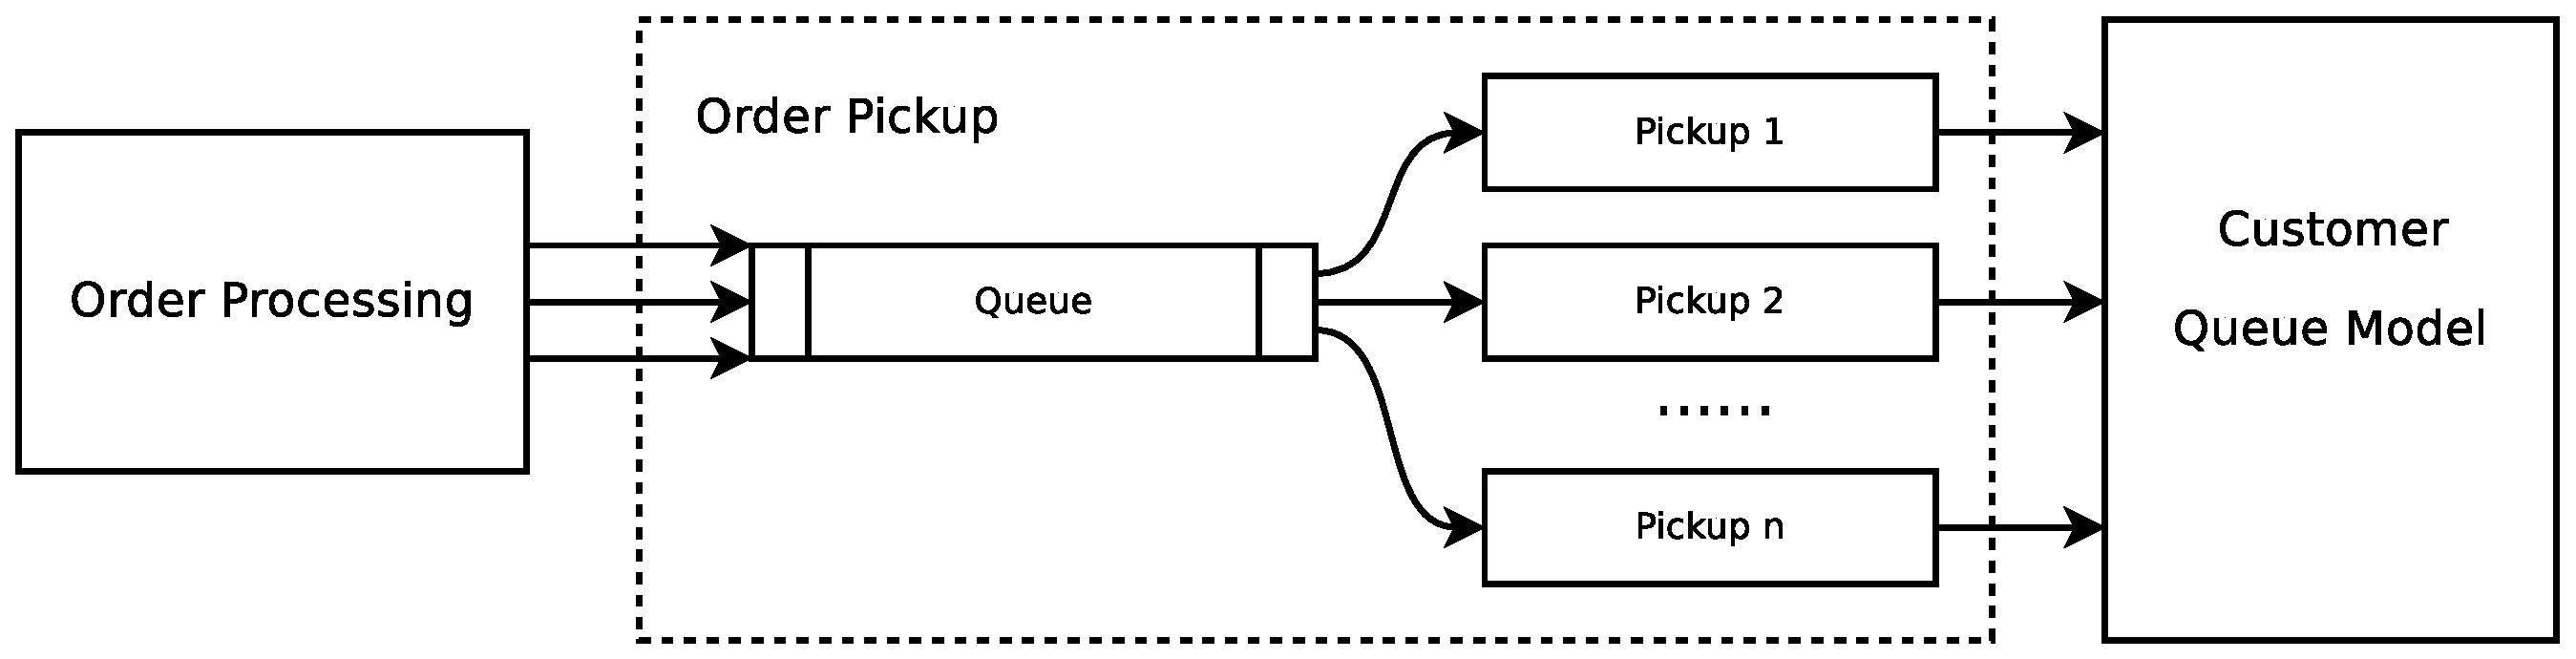
\includegraphics[width=0.60\textheight]{order_pickup}
	\caption{Order Pickup Part}
\end{figure}

Once an order is ready, it will be enqueued to order pickup part. The pickup part also has several pickup spaces with each pickup space occupied by at most one order at a given time. Also, the pickup spaces work in parallel independently. The orders in pickup spaces are dequeued from the pickup queue. Customers can only pickup the orders in pickup spaces but not in the pickup queue even if the orders are ready. The number of pickup spaces is designed to be as large as 10, so at most of the time, any order from processing part directly goes into pickup spaces without staying in pickup queue.

There is a small portion of time consumed in the order pickup. Usually, there is a pool of customers here waiting for pickup. The customers in the pool are not in any ordering. It is possible that the customer placed the latest order may be the first person to pickup in the pool. The time consumed in this part is assumed linear to the size of the pool to simulate the real Starbucks pickup. The formula is:
\[t=3\times\lfloor 0.1\times N+1\rfloor\]
where $N$ is the number of people in the pool. Thus, if there are less than 10 people in the pool, the pickup will take 3 seconds; if there are more than 10 to 19 people, the pickup consumes 6 seconds, and so on.

Notice that in certain customer queue model, this order pickup part may be missing (this is why it is in dash line). In some models we studied, the pickup is completed in the order placement part that each customer places the order and wait for pickup at the ordering window.

\newpage
\section{Customer Queue Models}

\subsection{Basic Model: One line with pickup}

Our basic model is the actual queuing model in Suzzallo Starbucks. There is only one lining queue for the order placement. Once any window finishes with a customer. The only line is dequeued. We impose a walking time from dequeuing to starting order at window. We assume the position where dequeuing happens is near the order placement window 1, so the customer walking to window 1 cost 1 second. The window 2 is a little bit further, so the customer walking to window 2 cost 2 seconds, and the time cost grows linearly as the window index increases.

In addition, there is a pickup area where customers can pickup their drinks when their orders are done. Any customers having finished order placement at window immediately enter a pool in pickup area where they are waiting for their order being processed. Other details are the same as described in 3.4 order pickup.

\subsection{Variation 1: One line without pickup}

From our basic model, we have our first variation. In this model, we still have people queuing up in one line for order placement but without pickup area. A customer will occupy an order placement window until his or her order is ready for pickup, or namely, the customer gets all the items he or she orders. During the time period after customer places his or her order and before his or her order is ready, the customer completely blocks the order placement window, but the cashier at the blocked window can now act as a worker to prepare the customer's order. Notice that the cashier can only prepare the order placed at his or her window, and will return to the window as long as that order is ready.

\subsection{Variation 2: Multiple lines with pickup}

In this model, we recover the pickup area setting in basic model, but this time there are separate lines for each window. If there are $n$ number of windows, then there are $n$ number of lining queues instead of one. In this setting, the time cost in walking to the window no longer grows as the window index. The time will fixed as 1 second.

\subsection{Variation 3: Multiple lines without pickup}

At this time, we combine the variation 1 and 2. We remove the pickup area, but keep the multiple line queuing model. The details of pickup area and multiple lines queuing are the same as described above.

\newpage
\section{Result \& Interpretation}

Analyzing the results from different variations of the model helps us understand the effect of each part of the queuing models, and gain insights to answer questions such as ``How to beat the line?'', and ``How to serve more customers in any given amount of time?'' 

\begin{figure}[H]
	\centering
	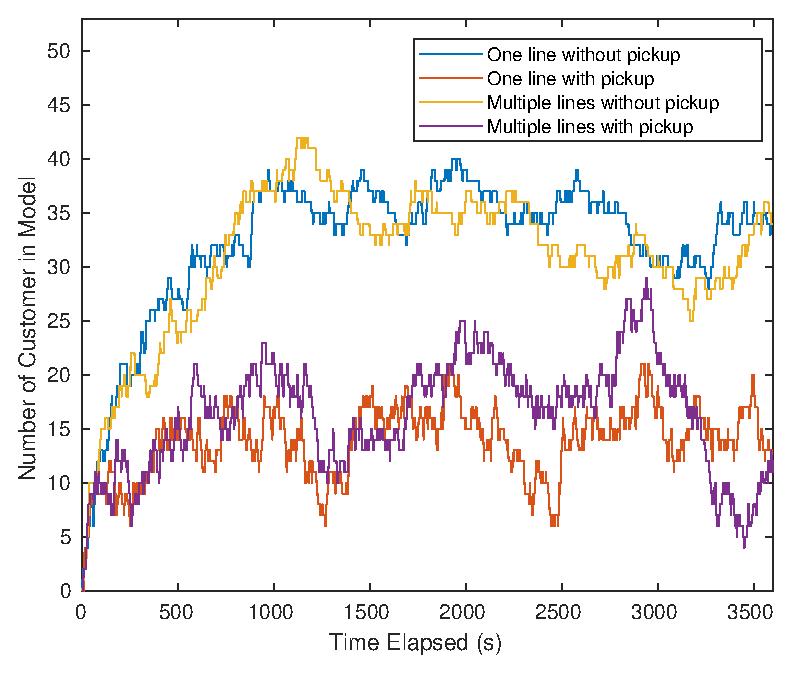
\includegraphics[width=0.35\textheight]{population_vs_time}
	\caption{Total Number of Customer in Model vs Time}
\end{figure}

In Figure 7, the four lines represent how the number of customers (both in ordering queue and pickup pool) change over a period of time (1 hour). The two lines on the top are models without pickup area, and the two lines at the bottom are models with pickup windows. From the graph, we can see that the models with the pickup process are significantly better in terms of reducing the number of customers waiting when comparing against models that does not separate the order and pickup process. This result is realistic since the customers waiting for items after ordering block the ordering window, which makes the ordering line longer and workers idle. 

\begin{figure}[H]
	\centering
	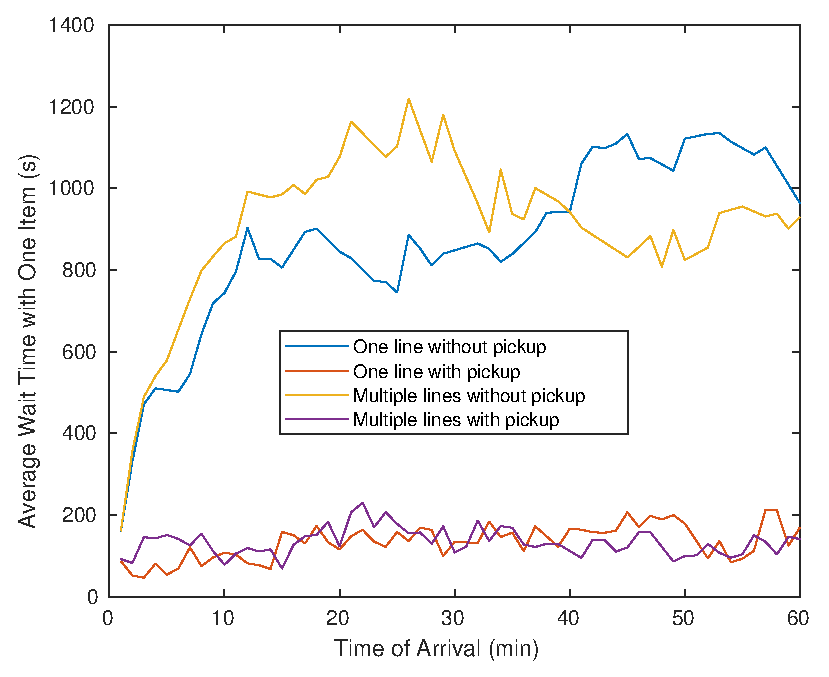
\includegraphics[width=0.35\textheight]{wait_time_one_item}
	\caption{Averaged Wait Time with One Item Ordered vs Enqueued Time}
\end{figure}

Figure 8 shows the averaged total wait time (for both ordering and pickup) one customer needs to wait if he or she only orders one item and arrives in different intervals of time. We discovered that the length of waiting time for the customers does not depend on the time they arrive (except at the beginning) when the model has a separate order and pickup process. However, the timing becomes critical when the order and pickup processes are combined.
At the beginning (time zero), there is no line and the customer waits for the least amount of time comparing to customers arriving later. In the course of one hour, two lines on the top (models without pickup windows) increases a lot in the first 20 minutes and then goes into equilibrium. Two lines on the bottom (models with pickup windows) shows no drastic changes. This result demonstrates the low efficiency of queues without pickup window, and that's why this kind of queue is rare in Starbucks.

\begin{figure}[H]
	\centering
	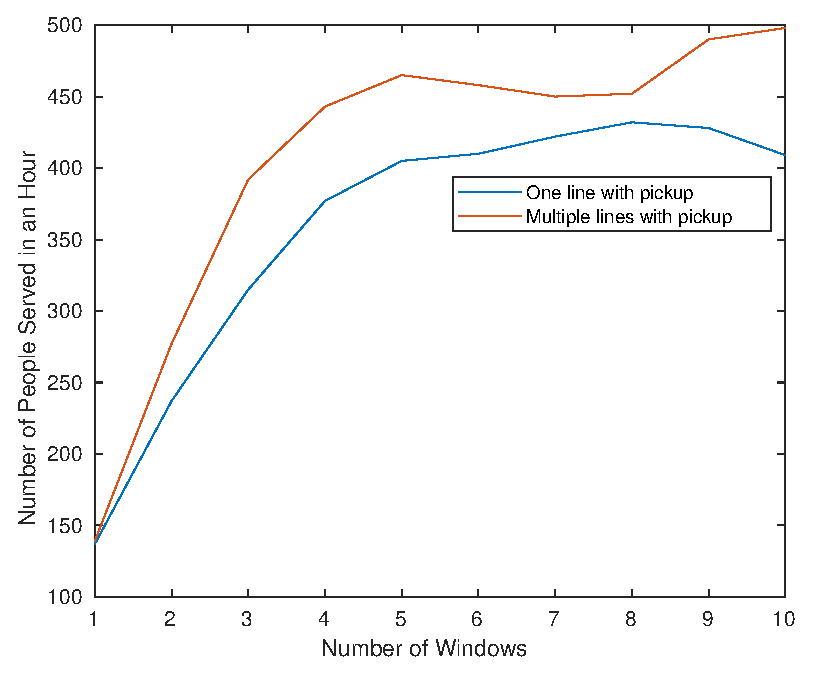
\includegraphics[width=0.35\textheight]{people_vs_window}
	\caption{Number of People Served in One Hour vs Number of Window}
\end{figure}

We can also make comments on how different customer queues and the efficiency of employees at Starbucks affect the model:

\begin{itemize}
\item One line vs. Multiple lines:\\
For the two ordering queues (one line for all customers vs. multiples lines for cashiers), Figure 9 demonstrates how the number of people being served in one hour changes as the number of windows increases. When there are multiple lines, the customer will choose the shortest line. The figure shows that the number of people being served by multiple lining queues is slightly greater than that by one line queue. Also, as the number of windows increases, the number of customers increases more in multiple lines queue. That's because it takes more time for customers to walk to each window if there is only one ordering line, and the walking time decreases the efficiency of the ordering process. Therefore, we conclude that for a Starbucks with many ordering windows, multiple lines for ordering would make the waiting time the least comparing to the other way of customer queue. In reality, most Starbucks use one line queue and we guess Starbucks' intention is to keep the line in order.

\item Pickup vs. No pickup:\\
The efficiency of the cashiers and workers determines the wait time for the customers, thus determining the most efficient queue model. When the workers are producing drinks efficiently, the order will be ready soon after it has been placed, so a pickup window is needed. When the cashiers are taking orders slowly, the processing queue never gets too long and workers can produce the drink and call out the customers one by one. Since the drinks will not queue up at the pickup desk, no pickup window for this model is needed.
\end{itemize}

\section{Adjustment \& Extension}

Our original model is using a varying $\lambda$ Poisson distribution to simulate balking. This kind of model is relatively complicated. At this time, we simplify the model to remove the balking setting. We assume that customers come at a constant rate of 0.2 person per second ($\lambda_0$ in original model).

\begin{figure}[H]
	\centering
	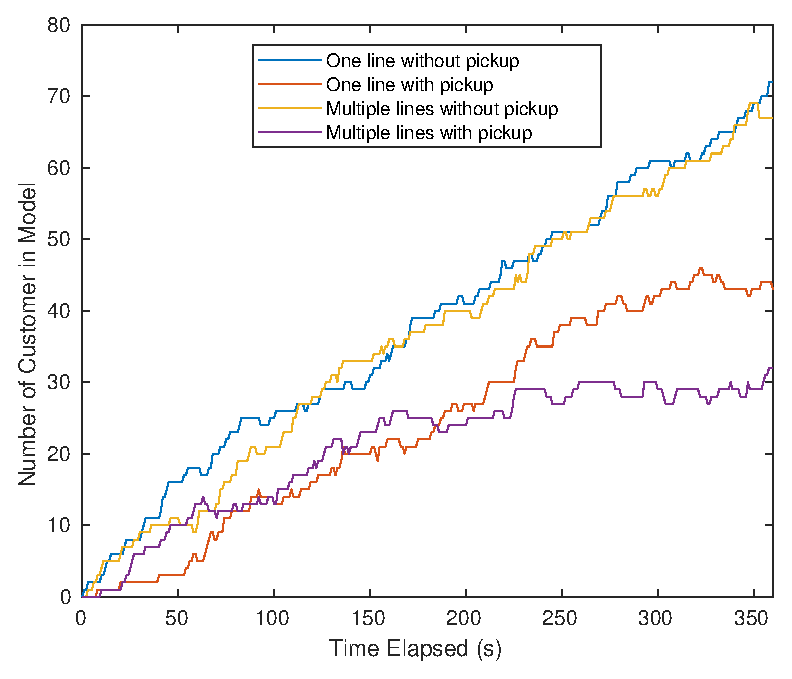
\includegraphics[width=0.40\textheight]{population_vs_time_ext}
	\caption{Total Number of Customer in Model vs Time (without balking)}
\end{figure}

\begin{figure}[H]
	\centering
	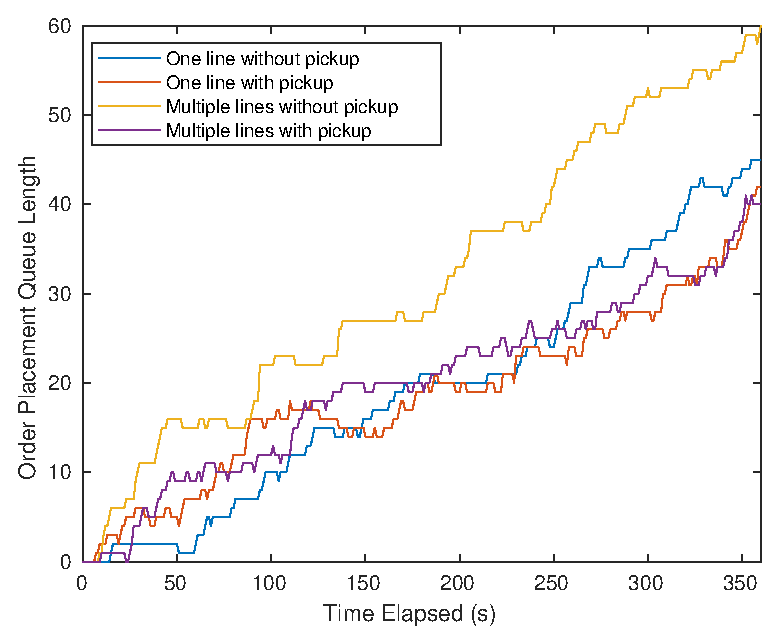
\includegraphics[width=0.40\textheight]{queue_length_vs_time_ext}
	\caption{Ordering Placement Queue Length vs Time (without balking)}
\end{figure}

As shown in the figure 10 and 11, without balking, the number of people both in the order placement queue and in the whole model steadily increase. In addition, the models without pickup area grow faster, because they are relatively inefficient as we discussed before.

\section{Conclusion}
Overall, our model simulates the actual scenarios at Suzzallo Starbucks closely: one ordering line, one order processing queue, and a pickup counter. The data collected substantiates our interpretation of the model and of the reality. Our model with different combinations of queuing methods enables us to make comments on the efficiency of queues.However, our model highly depends on assumptions we made. When we critically look at these assumptions we made throughout the model, we notice that some of them might be less supportive by reality or might not be representative. 

Firstly, in reality, there are more than 17 drinks in the Starbucks. We only choose the most popular 17 ones because they will have more effects on wait time comparing to the least popular ones. Also, customers can order "secrete recipe" with choices for the drink such as "tall decaf vanilla soymilk latte". Also, we use number one to five to rank the popularity of the drinks, but the actual popularity depends on season. In addition, our assumption that the popularity is proportional to the sale volume of the drink (drink with 5 popularity is 5 times more probable to be ordered than a drink with 1 popularity) is not exactly the same as reality because popularity of the drinks are usually not linear. Because people can read the reviews from other customers on each drink, the more a drink is ordered, the more people will order this drink. What's more, Starbucks also sells bakery, yogurt, and instant coffee, which prolongs the ordering time, and the bakery takes time for workers to toast.

Because of these limitations, we can further improve our model by introducing more choice of items and by eliminating some artificial assumptions in order to simulate the reality.

\newpage

\section*{Appendix}
All the code and data involved in this paper is shared on GitHub: \\
\url{https://github.com/liangyuRain/startbucks_queue_simulation} \\ \\

\noindent Survey Table \& Data collected:

\begin{center}
%	\includegraphics[width=0.40\textheight]{survey}
	\includegraphics[scale=0.6]{Survey_Summary}
\end{center}

\newpage
\bibliographystyle{alpha}
\bibliography{sample}

\end{document}